\documentclass[tikz,crop]{standalone}
%%% Tikz Libraries %%%
\usetikzlibrary{shapes.geometric}
\usetikzlibrary{positioning}

\begin{document}
  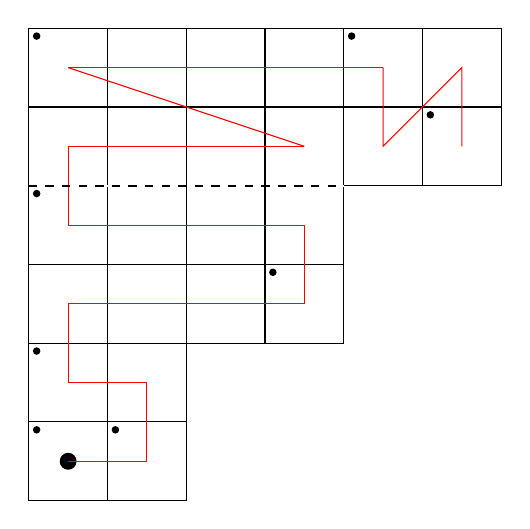
\begin{tikzpicture}
    %%% Mock Core Shape %%%
    % Row 1
    \draw[black] (1,1) rectangle (2,2); % 1
    \draw[black] (2,1) rectangle (3,2); % 2
    % Row 2
    \draw[black] (1,2) rectangle (2,3); % 3
    \draw[black] (2,2) rectangle (3,3); % 4
    % Row 3
    \draw[black] (1,3) rectangle (2,4); % 5
    \draw[black] (2,3) rectangle (3,4); % 6
    \draw[black] (3,3) rectangle (4,4); % 7
    \draw[black] (4,3) rectangle (5,4); % 8
    % Row 4
    \draw[black] (1,4) rectangle (2,5); % 9
    \draw[black] (2,4) rectangle (3,5); % 10
    \draw[black] (3,4) rectangle (4,5); % 11
    \draw[black] (4,4) rectangle (5,5); % 12
    % Row 5
    \draw[black] (1,5) rectangle (2,6); % 13
    \draw[black] (2,5) rectangle (3,6); % 14
    \draw[black] (3,5) rectangle (4,6); % 15
    \draw[black] (4,5) rectangle (5,6); % 16
    \draw[black] (5,5) rectangle (6,6); % 17
    \draw[black] (6,5) rectangle (7,6); % 18
    % Row 6
    \draw[black] (1,6) rectangle (2,7); % 19
    \draw[black] (2,6) rectangle (3,7); % 20
    \draw[black] (3,6) rectangle (4,7); % 21
    \draw[black] (4,6) rectangle (5,7); % 22
    \draw[black] (5,6) rectangle (6,7); % 23
    \draw[black] (6,6) rectangle (7,7); % 24

    %%% Ordered lines %%%
    \draw[fill=black] (1.5,1.5) circle (0.1);
    \draw[red] (1.5,1.5) -- (2.5,1.5) -- (2.5,2.5) -- (1.5,2.5);
    \draw[red] (1.5,2.5) -- (1.5,3.5) -- (3.5,3.5) -- (4.5,3.5);
    \draw[red] (4.5,3.5) -- (4.5,4.5) -- (3.5,4.5) -- (2.5,4.5) -- (1.5,4.5);
    \draw[red] (1.5,4.5) -- (1.5,5.5) -- (2.5,5.5) -- (3.5,5.5) -- (4.5,5.5);
    \draw[red] (4.5,5.5) -- (1.5,6.5);
    \draw[red] (1.5,6.5) -- (2.5,6.5) -- (3.5,6.5) -- (4.5,6.5) -- (5.5,6.5);
    \draw[red] (5.5,6.5) -- (5.5,5.5) -- (6.5,6.5) -- (6.5,5.5);

    %%% Draw reference nodes %%%
    \draw[fill=black] (1.1,1.9) circle (0.04);  % 1
    \draw[fill=black] (2.1,1.9) circle (0.04);  % 2
    \draw[fill=black] (1.1,2.9) circle (0.04);  % 3
    \draw[fill=black] (4.1,3.9) circle (0.04);  % 8
    \draw[fill=black] (1.1,4.9) circle (0.04);  % 9
    \draw[fill=black] (1.1,6.9) circle (0.04);  % 19
    \draw[fill=black] (5.1,6.9) circle (0.04);  % 23
    \draw[fill=black] (6.1,5.9) circle (0.04);  % 18

    %%% Draw Boundary %%%
    \draw[white,thick] (1,5) -- (5,5);
    \draw[black,dashed,thick] (1,5) -- (5,5);
  \end{tikzpicture}
\end{document}